\section{Introduction}

In the last years, recurrent neural networks, and particularly
long-short-term-memory (LSTM) architectures
\cite{Hochreiter:Schmidhuber:1997}, have been successfully applied to
a variety of challenging NLP tasks. This has spurred interest in
whether these generic sequence-processing devices are discovering
genuine structural properties of language in their training data, or
whether their success can be explained by opportunistic
heuristics. Starting with the seminal work of
\newcite{Linzen:etal:2016}, long-distance number agreement (``the
\textbf{boy} behind the trees \textbf{greets}\ldots'') has played a
central role in this debate. After mixed initial results by Linzen and
colleagues and \newcite{Bernardy:Lappin:2017},
\newcite{Gulordava:etal:2018} and \newcite{Kuncoro:etal:2018a} have
robustly established that LSTMs trained with the language modeling
objective on raw data achieve near-human performance on the
agreement task. While Gulordava and colleagues provided some evidence that the
LSTMs are relying on genuine syntactic generalizations,
\newcite{Kuncoro:etal:2018b} and \newcite{Linzen:Leonard:2018}
suggested that the LSTM achievements can, at least in part, be
accounted by superficial heuristics.

Until now, the debate has rested on ``behavioural'' evidence: The
LSTM is treated as a black box, and its capacities are indirectly
inferred by its performance on linguistic tasks. We take here a
complementary ``neuroscientific'' approach: We thoroughly investigate
the inner dynamics of an LSTM performing the number agreement task,
striving to achieve a mechanistic understanding of how it accomplishes
it.

We find that the LSTM specialized very few ``grandma'' cells
\cite{Bowers:2009} to carry number features from the subject to the
verb across the intervening material in a highly localist
fashion. Interestingly, the LSTM also possesses a more distributed
mechanism to predict number when subject and verb are close, with the
grandma number cells only playing a crucial role in more difficult
long-distance cases. Crucially, we independently identified a set of
cells tracking syntactic structure, and found that one of them \textcolor{red}{encodes the presence of an embedded phrase separating the main subject-verb dependency, and has} strong efferent connections to the long-distance number cells,
suggesting that the network relies on genuine syntactic information to
regulate agreement feature percolation.

Our analysis thus provides direct evidence for the claim that LSTMs
trained with language modeling on unannotated corpus data, despite
lacking significant linguistic priors, learn to perform
structure-dependent linguistic operations. In turn, this suggests that
raw linguistic input and generic memory mechanisms, such as those
implemented in the LSTM, might suffice to trigger the induction of
non-trivial grammatical rules.

\textbf{The following fragments should probably go in the
  conclusion. I'm not sure of where the bit on the plural/singular
  asymmetry should go (I don't think we should emphasize the
  ``behavioural'' part of it, as that's tangential to the main story in
  this paper).}

More generally, we provided the most detailed analysis of the inner
dynamics of an LSTM performing a linguistic task we are aware of. We
think that similar studies should complement currently popular
black-box tests, to achieve a true understanding of language
processing in neural networks. \textbf{Here, we might want to mention
  the need for future work on relative clauses, as well as on other
  models, such as transformers.}

From a more cognitive perspective, we hope our granular
understanding of how LSTMs perform number agreement will inform work
on computational modeling of neural sentence processing data, as we
conjecture a similar interaction between syntactic and
feature-carrying units might be implemented in the human
brain. Intriguingly, we observed differential handling of singular and
plural information, with the latter being more reliably processed,
resulting in more robust plural agreement. As a similar asymmetry has
also been observed in humans (\textbf{REFS}), one exciting avenue for
future work might consist in looking for different singular/plural
processing networks in the human brain.


\begin{figure}
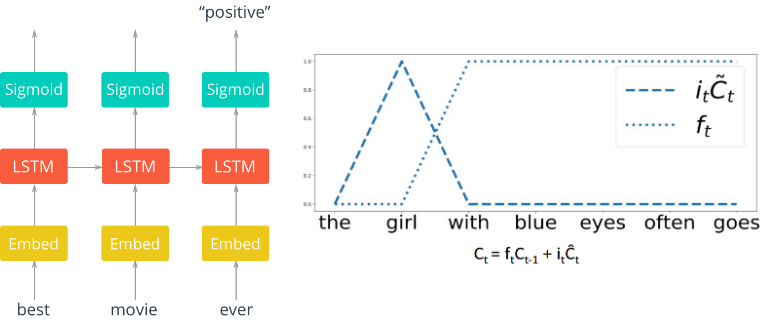
\includegraphics[width=\linewidth]{Figures/Figure1_intro.png}
\caption{Caption.}
\end{figure}
